\documentclass{beamer}

\usepackage[spanish]{babel}
\usepackage[utf8]{inputenc}
\usepackage{comment}
\usepackage{color}
\usepackage{pdfpages}
\usepackage{amsmath}
\usepackage{appendixnumberbeamer}
\usepackage{ragged2e}

\usetheme{Rochester}
\usecolortheme{beaver}
\usefonttheme{structurebold}
\setbeamertemplate{footline}[frame number]
\setbeamertemplate{navigation symbols}{}

\title{Hiding in the Crowd}
\subtitle{Design and Implementation of a DC-Net-based\\Anonymous Messaging System}

\author{Camilo José Gómez Núñez}

\institute[]
{Departamento de Ciencias de la Computación\\
Facultad de Ciencias Físicas y Matemáticas\\
Universidad de Chile}

\date{June, 28th 2018}

\AtBeginSection[]
{
  \begin{frame}<beamer>{Outline}
    \tableofcontents[currentsection]
  \end{frame}
}

\begin{document}

\begin{frame}
  \titlepage
\end{frame}

{
\setbeamercolor{background canvas}{bg=black}
\begin{frame}[plain]
\vspace{4.45em}
\begin{center}
\only<1>{\textbf{\color{red}\fontfamily{cmtt}\selectfont\Huge{A N O N Y M I T Y}}}
%\only<2>{\textbf{\color{red}\fontfamily{cmtt}\selectfont\Huge{(n -) A N O N Y M I T Y}}}
%\only<3->{\textbf{\color{red}\fontfamily{cmtt}\selectfont\Huge{A N O N Y M I T Y}}}

%\only<4->{\color{red}\rule{20em}{1pt}}

%\only<4->{\textbf{\color{red}\fontfamily{cmtt}\selectfont\Huge{\rotatebox{180}{Y T I M Y N O N A}}}}
\end{center}
\end{frame}
}

\begin{frame}{Anonymity today}
    \centering
    \includegraphics<2>[scale=0.17]{images/tor.png}
\end{frame}

\begin{frame}{Thesis' Objective}
\justify
\huge{Provide an \textbf{alternative system to \emph{TOR}} that would be useful in some bounded scenarios that doesn't possess the limitations that \emph{onion-routing} has.}
\end{frame}

\begin{frame}{Contents}
  \tableofcontents
\end{frame}

\begin{frame}{Comparison between TOR and DC-NET}

\begin{table}[]
\centering
\begin{tabular}{l|l|l|}
\cline{2-3}
                                      & \multicolumn{1}{c|}{\textbf{ADVANTAGES}}                                                                                     & \multicolumn{1}{c|}{\textbf{DISADVANTAGES}}                                                                             \\ \hline
\multicolumn{1}{|c|}{\textbf{TOR}}    & \begin{tabular}[c]{@{}l@{}}- Fast.\\ - Scalable.\end{tabular}                                                                & \begin{tabular}[c]{@{}l@{}}- Insecure against \\   global adversary.\\ - Need trust in third \\   parties.\end{tabular} \\ \hline
\multicolumn{1}{|l|}{\textbf{DC-NET}} & \begin{tabular}[c]{@{}l@{}}- Secure against \\   global adversary.\\ - Doesn't need trust\\   in third parties.\end{tabular} & \begin{tabular}[c]{@{}l@{}}- Robustness. (?)\\ - Efficiency. (?)\end{tabular}                                           \\ \hline
\end{tabular}
\end{table}

\end{frame}

\section{Introduction}

\begin{frame}{General DC-NET}

\frametitle<1-3>{General DC-NET - Objective}
\vspace{2em}
\centering
\includegraphics<1-1>[scale=0.5]{images/dcnet-general-test-0.png}
\includegraphics<2-2>[scale=0.5]{images/dcnet-general-test-1.png}
\includegraphics<3-3>[scale=0.5]{images/dcnet-general-test.png}
\includegraphics<4-4>[scale=0.5]{images/dcnet-general-test-2.png}
\includegraphics<5-5>[scale=0.5]{images/dcnet-general-test-3.png}

\frametitle<4->{General DC-NET}
\begin{columns}<6->[c]
    \column{.5\textwidth}
    \centering
    \includegraphics[scale=0.4]{images/dcnet-general-test-3.png}
    \vspace{.5cm}
    \setbeamercolor{postit}{fg=black,bg=yellow}
    \begin{beamercolorbox}[sep=1em,wd=3cm,center]{postit}
        $K_{ij} = -K_{ji}$
    \end{beamercolorbox}
    \column{.5\textwidth}
    \centering
    \begin{block}{Output Messages}
      \footnotesize
      \begin{itemize}
      \setlength{\itemindent}{-.25in}
          \item[]<7-> \textcolor{blue}{$O_A = K_{ab} + K_{ac} + K_{ad} + K_{ae}$}
          \item[]<8-> \textcolor{green}{$O_B = K_{ba} + K_{bc} + K_{bd} + K_{be}$ + \textbf{\textcolor{black}{$M$}}}
          \item[]<9-> \textcolor{orange}{$O_C = K_{ca} + K_{cb} + K_{cd} + K_{ce}$}
          \item[]<10-> \textcolor{yellow}{$O_D = K_{da} + K_{db} + K_{dc} + K_{de}$}
          \item[]<11-> \textcolor{red}{$O_E = K_{ea} + K_{eb} + K_{ec} + K_{ed}$}
      \end{itemize}
    \end{block}
    
    \begin{exampleblock}<12->{Obtain Message}
    \centering
    $C = \sum O_i = M$
    \end{exampleblock}
\end{columns}

\end{frame}

% \begin{frame}{DC-NET Robustness Problems}
    
    \begin{alertblock}{Cheating}
        Malicious participants send incorrect values in their output messages.
    \end{alertblock}
    
    \begin{alertblock}{Collision}
        More than one participant send a message in their output messages.
    \end{alertblock}
    
\end{frame}

\section{Design of a Robust DC-NET Variant}

\begin{frame}{DC-NET Robustness Problems}
    
    \begin{alertblock}{Cheating}
        Malicious participants send incorrect values in their output messages.
    \end{alertblock}
    
    \begin{alertblock}{Collision}
        More than one participant send a message in their output messages.
    \end{alertblock}
    
\end{frame}

\begin{frame}{Real Round - Key-Sharing}
    \begin{columns}[c]
        \column{.5\textwidth}
            \hspace{-0.9cm}
            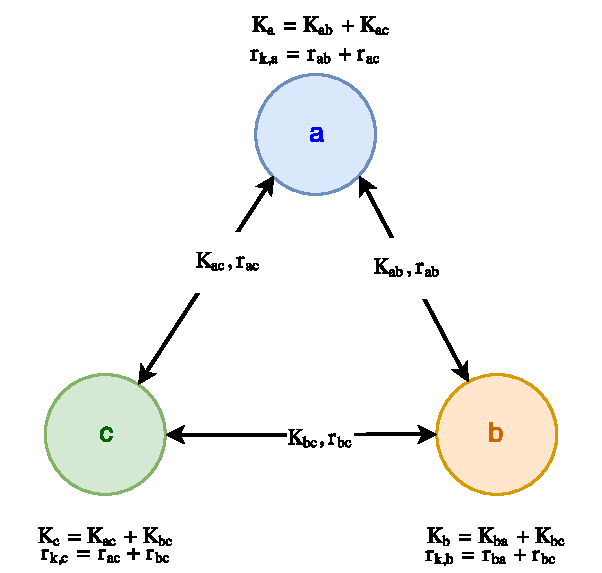
\includegraphics[scale=.6]{images/keys-sharing.pdf}
            \vspace{.2cm}
            \setbeamercolor{postit}{fg=black,bg=yellow}
            \centering
            \begin{beamercolorbox}[sep=.5em,wd=3cm,center]{postit}
                $K_{ij} = -K_{ji}$\\
                $r_{ij} = -r_{ji}$
            \end{beamercolorbox}
        \column{.5\textwidth}
            \begin{block}<2->{Commitments on Keys}
                \centering
                $c_{k,a} = g^{K_a} h^{r_{k,a}}$\\
                $c_{k,b} = g^{K_b} h^{r_{k,b}}$\\
                $c_{k,c} = g^{K_c} h^{r_{k,c}}$
            \end{block}
            \begin{block}<3->{PoK on Keys}
                \centering
                \scriptsize$\mathtt{PoK}_{k,a} = PoK\{(K_a, r_{k,a}): c_{k,a} = g^{K_a} h^{r_{k,a}}\}$\\
                \scriptsize$\mathtt{PoK}_{k,b} = PoK\{(K_b, r_{k,b}): c_{k,b} = g^{K_b} h^{r_{k,b}}\}$\\
                \scriptsize$\mathtt{PoK}_{k,c} = PoK\{(K_c, r_{k,c}): c_{k,c} = g^{K_c} h^{r_{k,c}}\}$\\
            \end{block}
            \begin{exampleblock}<4->{Check values}
                \centering
                $\prod c_{k,i} \overset{?}{=} 1$
            \end{exampleblock}
    \end{columns}
\end{frame}
\begin{frame}{DC-NET Robustness Problems}
    
    \begin{exampleblock}{Cheating}
        Malicious participants send incorrect values in their output messages.
    \end{exampleblock}
    
    \begin{alertblock}{Collision}
        More than one participant send a message in their output messages.
    \end{alertblock}
    
\end{frame}
\begin{frame}{General DC-NET}

\begin{columns}[c]
    \column{.5\textwidth}
    \centering
    \includegraphics[scale=0.4]{images/dcnet-general-03.png}
    \vspace{.5cm}
    \setbeamercolor{postit}{fg=black,bg=yellow}
    \begin{beamercolorbox}[sep=1em,wd=3cm,center]{postit}
        $K_{ij} = -K_{ji}$
    \end{beamercolorbox}
    \column{.5\textwidth}
    \centering
    \begin{block}{Output Messages}
      \footnotesize
      \begin{itemize}
      \setlength{\itemindent}{-.25in}
          \item[] \textcolor{blue}{$O_A = K_{AB} + K_{AC} + K_{AD} + K_{AE} + M_1$}
          \item[] \textcolor{green}{$O_B = K_{BA} + K_{BC} + K_{BD} + K_{BE} + M_2$}
          \item[] \textcolor{orange}{$O_C = K_{CA} + K_{CB} + K_{CD} + K_{CE} + M_3$}
          \item[] \textcolor{yellow}{$O_D = K_{DA} + K_{DB} + K_{DC} + K_{DE} + M_4$}
          \item[] \textcolor{red}{$O_E = K_{EA} + K_{EB} + K_{EC} + K_{ED} + M_5$}
      \end{itemize}
    \end{block}
    
    \begin{exampleblock}{Obtain Message}
    \centering
    $C = \sum O_i = M_1 + M_2 + M_3 + M_4 + M_5$
    \end{exampleblock}
\end{columns}

\end{frame}
\begin{frame}{Collision Resolution Example}
    \centering
    \includegraphics<1-1>[scale=.4]{images/collision-resolution-example-01.pdf}
    \includegraphics<2-2>[scale=.4]{images/collision-resolution-example-02.pdf}
    \includegraphics<3-3>[scale=.4]{images/collision-resolution-example-03.pdf}
    \includegraphics<4-4>[scale=.4]{images/collision-resolution-example-04.pdf}
    \includegraphics<5-5>[scale=.4]{images/collision-resolution-example-05.pdf}
    \includegraphics<6-6>[scale=.4]{images/collision-resolution-example-00.pdf}
\end{frame}
\begin{frame}{Real Round - $M_i$ Format - Identify Collisions}
    \centering
    If participant $P_i$ will send a message in this round, $M_i$:
    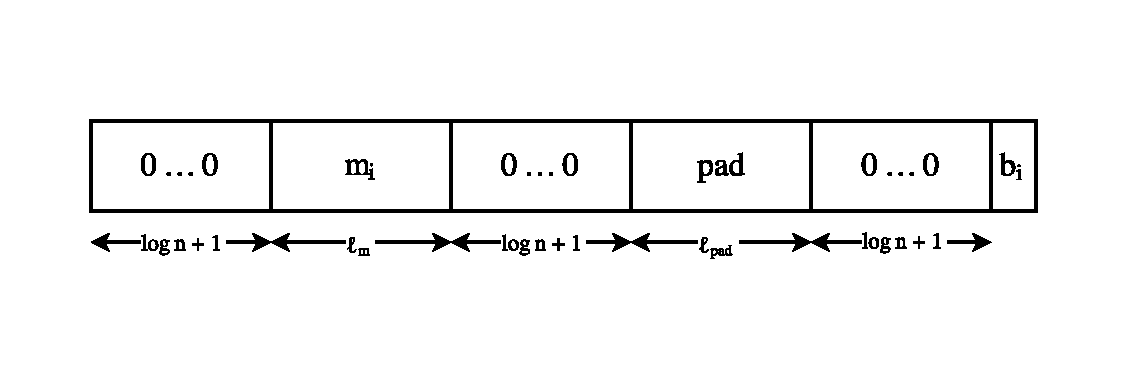
\includegraphics[scale=.55]{images/message-format(1).pdf}\\
    If not, $M_i$:
    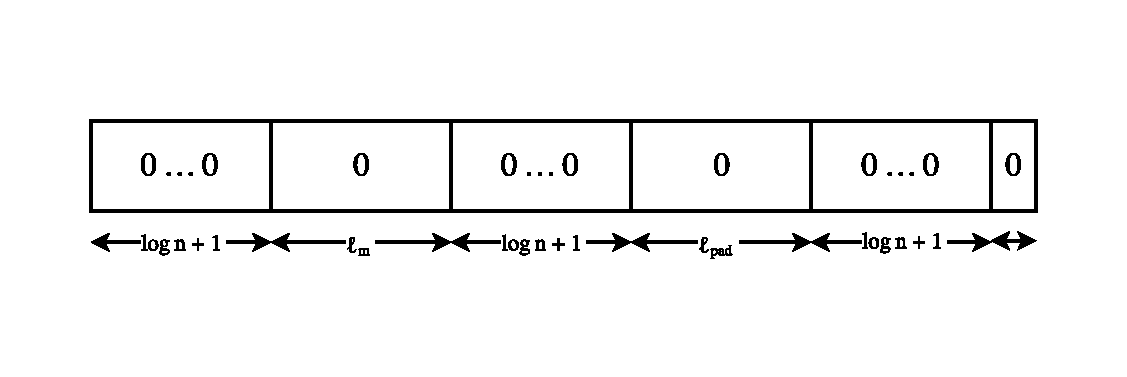
\includegraphics[scale=.55]{images/message-format-nomessage.pdf}
\end{frame}
%\begin{frame}{Real Round - Message $M_i$ Format Proof}
    \begin{block}<1->{Informal Property}
        Participant must prove that is sending a message ($b_i = 1$) or no message at all ($b_i = 0 \land m_i = 0$). 
    \end{block}
    \begin{block}<2>{Data Sending}
        $P_i$ chooses randomly: $r_m, r_b, r_{\mathtt{pad}}$\\
        $P_i$ calculates: $c_m = g^{m_i} h^{r_m}, c_b = g^{b_i} h^{r_b}, c_{\mathtt{pad}} = g^{\mathtt{pad}_i} h^{r_{\mathtt{pad}}}$\\
        $P_i$ generates: $\mathtt{PoK}_{\mathtt{format}} = PoK\{(r_m, r_b): (g^{-1} c_b = h^{r_b}) \lor (c_b = h^{r_b} \land c_m = h^{r_m})\}$\\
        $P_i$ sends the proof and the commitments, and with all that the rest of the participants can check that the proof is valid.
    \end{block}
\end{frame}
%
%\begin{frame}{Real Round - Message values}
    \begin{block}<1->{Sending message in current round}
    $m_i = m$; plain message to send\\
    $\texttt{pad}_i \stackrel{\$}{=} \texttt{pad}$\\
    $b_i = 1$\\
    $O_i = M_i + K_i$
    \end{block}
    \begin{block}<2>{No message in this round}
    $m_i = 0$\\
    $\texttt{pad}_i = 0$\\
    $b_i = 0$\\
    $O_i = K_i$
    \end{block}
\end{frame}
%
%\begin{frame}{Real Round - Proof of Knowledge on $M_i$}
    \begin{block}<1->{Informal Property}
        Participant will generate a commitment for $M_i$ using the commitments created in the previous step, and with that a PoK for the message $M_i$ inside that commitment.
    \end{block}
    \begin{block}<2>{Data Sending}
        $P_i$ calculates $c_M = f(c_m, c_b, c_\mathtt{pad})$\\
        $P_i$ extracts the value $r_M$ inside $c_M$ calculated before.\\
        $P_i$ generates: $\mathtt{PoK}_M = PoK\{(M, r_M): c_M = g^{M} h^{r_M}\}$\\
        $P_i$ sends the proof, and the rest of the participants need to check that the proof is valid using the commitments received in the previous step.
    \end{block}
\end{frame}
%\begin{frame}{Real Round - Sending $O_i$ in round 1}
    \begin{block}{Informal Property}
        Participant generates a commitment and a PoK for $O_i$ (established before), and the rest of the participants will check the proof using the values of commitments received in previous steps. $P_i$ will send this proof and the value $O_i$ itself.
        
        After that, each $O_i$ of the participants will be added in order to construct the round message $C^{(1)}$.
    \end{block}
\end{frame}

\begin{frame}{Real Round - Sending $O_i$ in round 1}
    \begin{block}{Data Sending}
        $P_i$ calculates $r_{O} = r_{M} + r_{K}$\\
        Then calculates the commitment $c_{r_O} = h^{r_O}$\\
        Generates $\mathtt{PoK_{r_O}} = PoK\{r_O:c_{r_O} = h^{r_O}\}$ and sends it along $O_i$ to the rest of the room.\\
        The rest of participants calculate commitment for each $O_j$ received as $c_O = c_K \cdot c_M$\\
        After this will calculate the value $\beta = c_O \cdot (g^O)^{-1}$, and with this value will verify $\mathtt{PoK_{r_O}}$\\
        Finally will calculate $C^{(1)} = \sum O_j$
    \end{block}
\end{frame}
%\begin{frame}{Real Round - Sending $O_i$ when father round is real}
    \begin{block}<1-1>{Informal Property}
        Participant sends $O_i$ and a proof verifying that the message is either 0 or is the same message that was involved in the collision in the father round.
        
        Same as before, all $O_i$ will be added in order to construct the round message $C^{(k)}$
    \end{block}
\end{frame}

\begin{frame}{Real Round - Sending $O_i$ when father round is real}
    \centering
    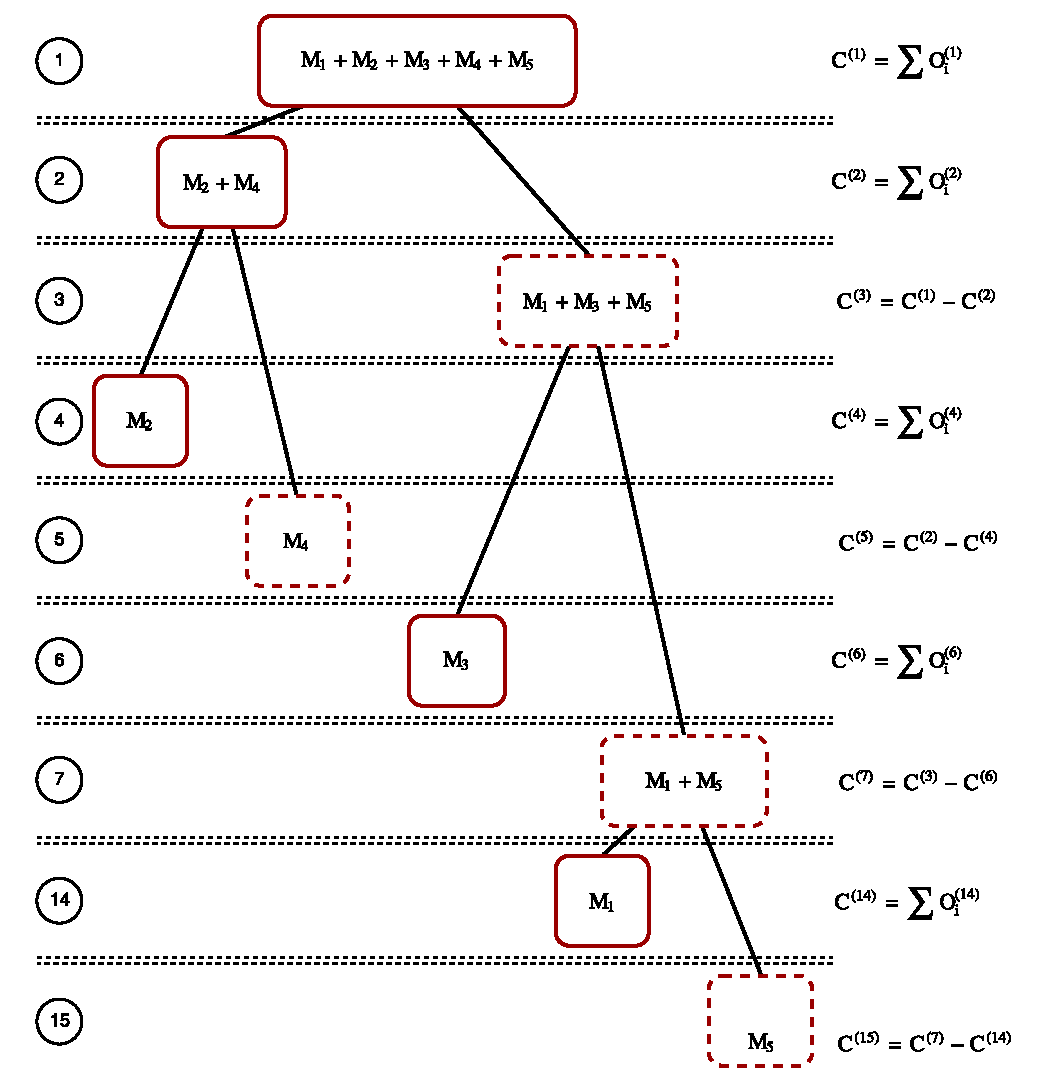
\includegraphics[scale=.4]{images/collision-resolution-example-00.pdf}
\end{frame}
%\begin{frame}{Real Round - Sending $O_i$ when father round is virtual}
    \begin{block}{Informal Property}
        Participant sends $O_i$ and a proof verifying that the message is either 0 or is the same message that was involved in the last real round played in the direct branch between the current round and the first one. Also needs to prove that this message wasn't involved in real rounds produced in later real rounds of other branches.
        
        Same as before, all $O_i$ will be added in order to construct the round message $C^{(k)}$
    \end{block}
\end{frame}

\begin{frame}{Real Round - Sending $O_i$ when father round is virtual}
    \centering
    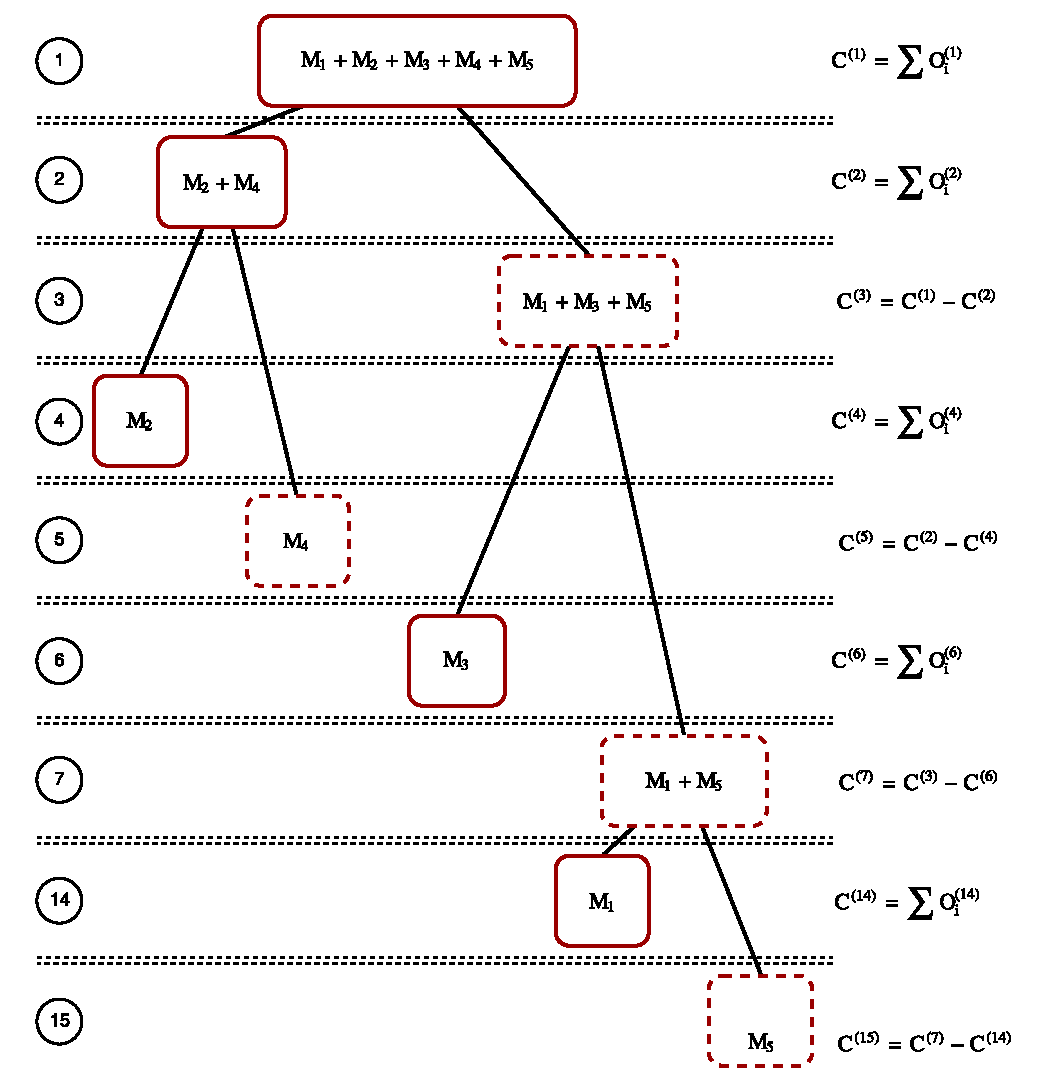
\includegraphics[scale=.4]{images/collision-resolution-example-00.pdf}
\end{frame}


\begin{frame}{Real Round $k$ Summary}
    \begin{enumerate}
        \item Key Exchange.
        \item Construct Message $M_i$.
        \item Proof for correct format of $M_i$.
        \item Proof of Knowledge on $m_i$.
        \item $O_i$ sending along with correctness proof.
        \item Construct round message $C^{(k)}$
        \item Round Resolution (collision or single message reception).
    \end{enumerate}
\end{frame}

\begin{frame}{DC-NET Robustness Problems}
    
    \begin{exampleblock}{Cheating}
        Malicious participants send incorrect values in their output messages.
    \end{exampleblock}
    
    \begin{exampleblock}{Collision}
        More than one participant send a message in their output messages.
    \end{exampleblock}
    
\end{frame}
%\begin{frame}{Virtual Round}
    \begin{block}{Steps to obtain resulting round message}
        \begin{enumerate}
            \item Retrieve $C^{(k)}$ and $C^{(2k)}$
            \item Calculate $C^{(2k+1)} = C^{(k)} - C^{(2k)}$
        \end{enumerate}
    \end{block}
\end{frame}
%\begin{frame}{Round Resolution - Message Split}
    \begin{block}{Round message splitting}
        Separate $C^{(k)}$ in the pair $(M^*, t)$, where:\\
        $M^*$ is the sum of all messages sent by each of the participants, and\\
        $t$ is the number of messages involved in the collision.
    \end{block}
\end{frame}
%\begin{frame}{Round Resolution - Collision Size}
    \begin{block}{First Collision}
        In round 1, the first collision size $N$ is established. After $N$ real rounds, this collision will be resolved, thus finishing the current session.\\
        If $N = 0$, no message was sent.\\
    \end{block}
\end{frame}
%\begin{frame}{One Message Round - No Collision}
    \begin{block}{$t = 1$}
        When $t = 1$, only one message is sent in this round, so we need to increase the number of messages received in the session. When this number reaches $N$, the session is over (the first collision was resolved completely).
    \end{block}
\end{frame}
%\begin{frame}{Collision Round}
    \begin{block}{$t > 1$}
        All the participants that sent a message in this round need to calculate: $\overline{M} = M^*/t$\\
        If his message $M_i < \overline{M}$, will resend his message in the round $2k$\\
        If not, the participant will resend his message in the round $2k+1$ (which is virtual, so technically won't resend his message).
    \end{block}
    \begin{block}<2>{Aftermath}
        The current round is over, and a new round (if it is the case) will start, redoing all the previous steps described.
    \end{block}
\end{frame}

\begin{frame}{Comparison between TOR and DC-NET}

\begin{table}[]
\centering
\begin{tabular}{l|l|l|}
\cline{2-3}
                                      & \multicolumn{1}{c|}{\textbf{ADVANTAGES}}                                                                                     & \multicolumn{1}{c|}{\textbf{DISADVANTAGES}}                                                                             \\ \hline
\multicolumn{1}{|c|}{\textbf{TOR}}    & \begin{tabular}[c]{@{}l@{}}- Fast.\\ - Scalable.\end{tabular}                                                                & \begin{tabular}[c]{@{}l@{}}- Insecure against \\   global adversary.\\ - Need trust in third \\   parties.\end{tabular} \\ \hline
\multicolumn{1}{|l|}{\textbf{DC-NET}} & \begin{tabular}[c]{@{}l@{}}- Secure against \\   global adversary.\\ - Doesn't need trust\\   in third parties.\end{tabular} & \begin{tabular}[c]{@{}l@{}}- Robustness. (\checkmark)\\ - Efficiency. (?)\end{tabular}                                           \\ \hline
\end{tabular}
\end{table}

\end{frame}

\section{Implementation Details}

\begin{frame}{Software Tools}
    \begin{itemize}
        \item Java language
        \item ZeroMQ
        \item Crypto libraries
        \item API Implemented
    \end{itemize}
\end{frame}
\begin{frame}{System Architecture - Directory Node}
    \centering
    \includegraphics<1-1>[scale=.6]{images/architecture.pdf}
\end{frame}
\begin{frame}{System Architecture - Participants Connection}
    \centering
    \includegraphics<1-1>[scale=.6]{images/participants_connection.pdf}
\end{frame}
\input{20_implementation_cryptography}
\begin{frame}{API for Mobile App}
    
    \begin{block}{API Functions}
        \begin{itemize}
            \item \texttt{connectToDirectory()}
            \item \texttt{ObservableParticipantsLeft}
            \item \texttt{setMessage()}
            \item \texttt{runProtocol()}
            \item \texttt{ObservableMessagesArrived}
        \end{itemize}
    \end{block}

\end{frame}

\begin{frame}{API for Mobile App}
    \begin{columns}[c]
        \column{.5\textwidth}
        \centering
        \includegraphics[scale=0.15]<1-1>{images/mobile_first.png}
        \includegraphics[scale=0.15]<2-2>{images/mobile_connecting.png}
        
        \column{.5\textwidth}
        \centering
        \includegraphics[scale=0.15]<1-1>{images/mobile_connect.png}
        \includegraphics[scale=0.15]<2-2>{images/mobile_message.png}
    
    \end{columns}
\end{frame}
\section{Experiments}

\begin{frame}{Experiments - Experimental Design}
    
    \begin{block}{Preliminary Setting}<1->
        \begin{itemize}
            \item \emph{Common Open Research Emulator (CORE)}
            \item 30 Participants node, 1 Directory node
            \item Local Network parameters
            \item 2 experiments: fixed anonymity-set and variable anonymity-set
        \end{itemize}
    \end{block}
    
    \begin{block}{Experiments}<2>
        \begin{itemize}
            \item Stages Profile
            \item Protocol Bandwidth
            \item Execution times: total, first message and average per round
        \end{itemize}
    \end{block}
    
\end{frame}
\begin{frame}{Experiments - Results - Stages Profile}
    \makebox[\linewidth][c]{%
        \begin{minipage}{\dimexpr\textwidth+4.8em\relax}
        \raggedright
        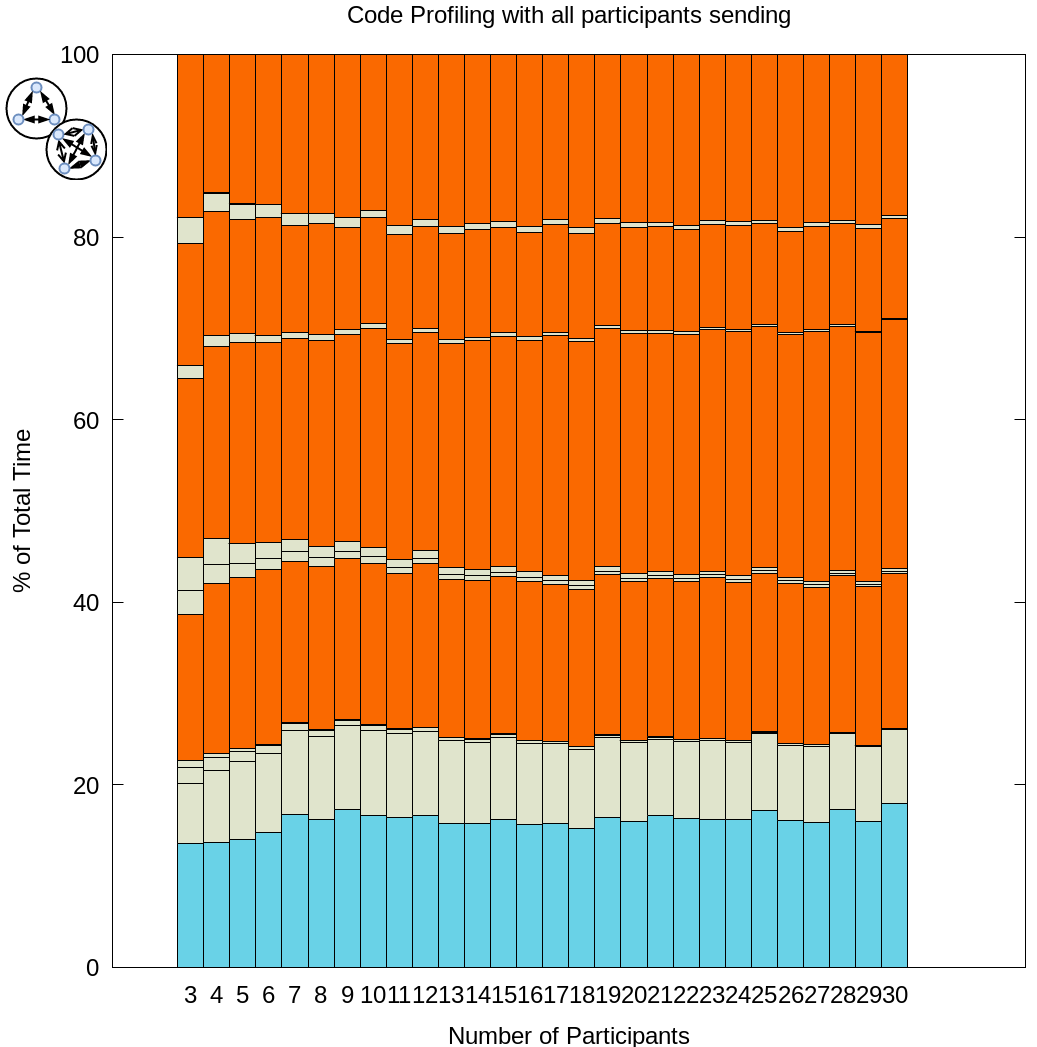
\includegraphics[scale=0.13]{images/profile_all.png}
        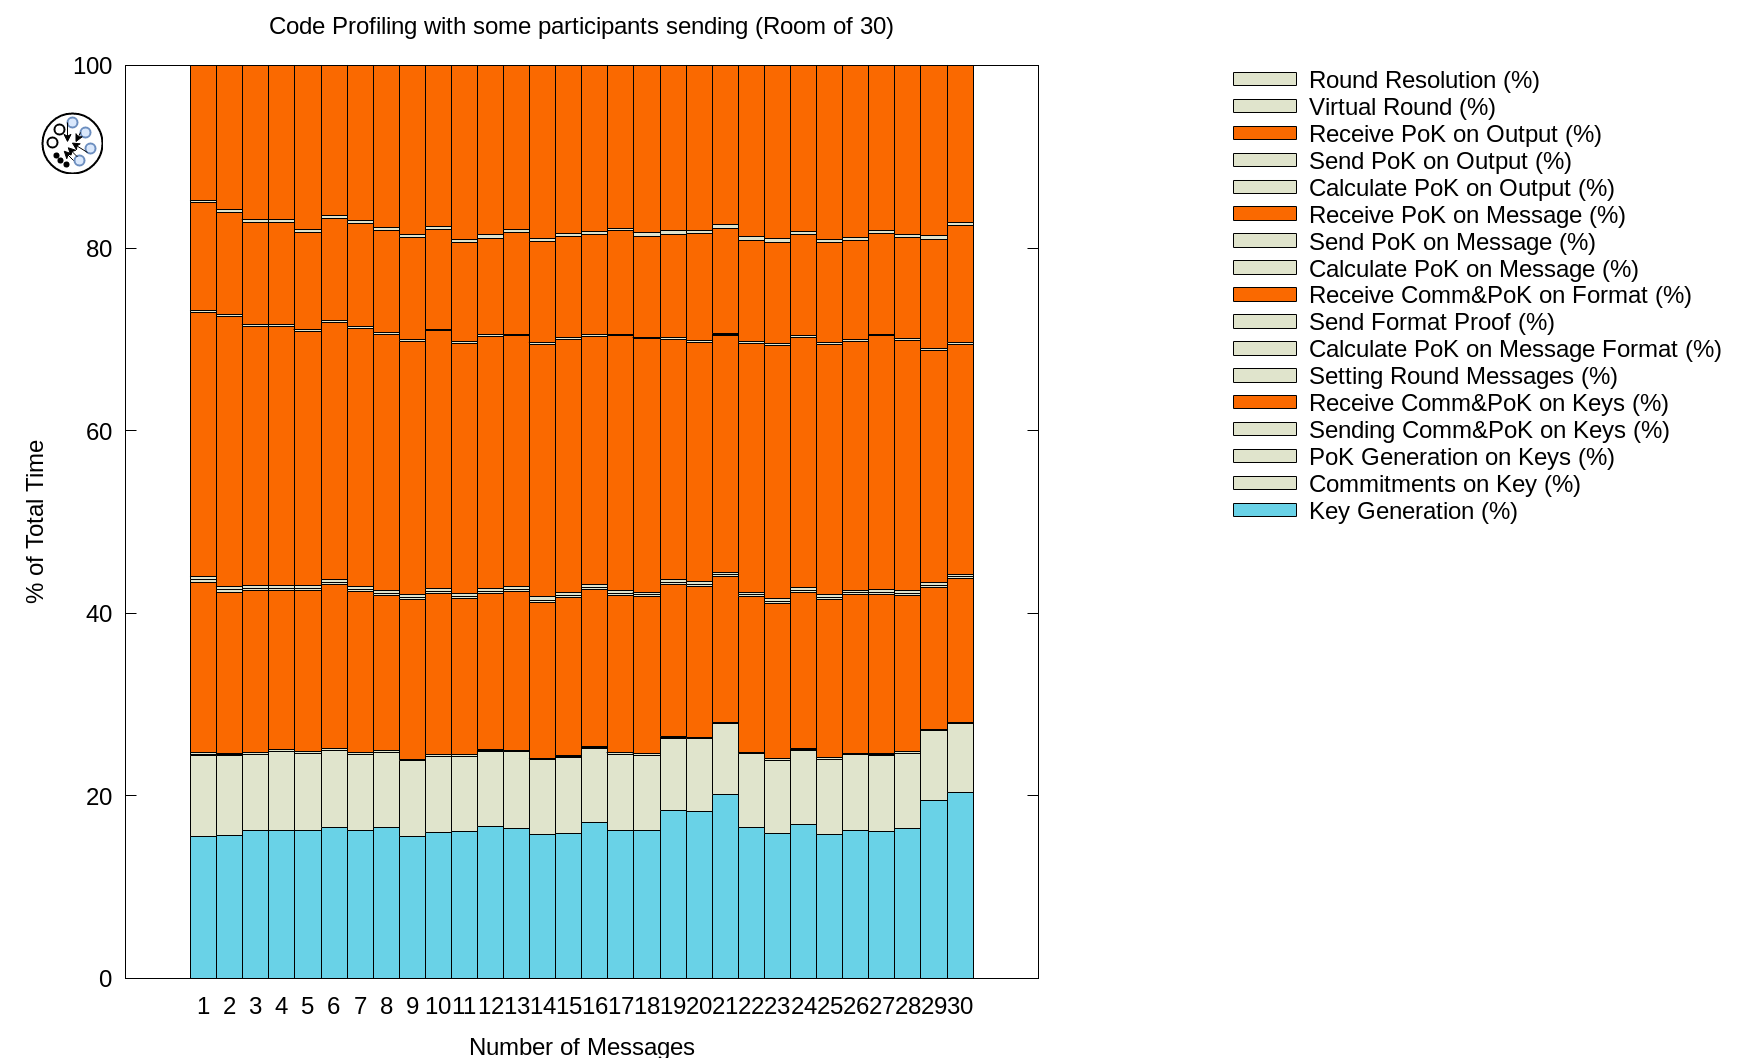
\includegraphics[scale=0.13]{images/profile_partial.png} \end{minipage}%
    }%
\end{frame}

\begin{frame}{Protocol Bandwidth}
    \centering
    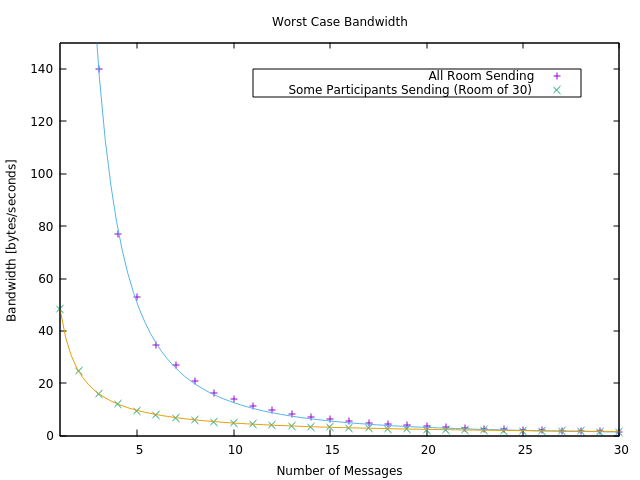
\includegraphics[scale=0.6]{images/bandwidth.png}
\end{frame}

\begin{frame}{Experiments - Results - Execution Time}
    \centering
    \includegraphics<1-1>[scale=0.3]{images/fixed_room.png}
    \includegraphics<2>[scale=0.3]{images/variable_room.png}
\end{frame}

\begin{frame}{Comparison between TOR and DC-NET}

\begin{table}[]
\centering
\begin{tabular}{l|l|l|}
\cline{2-3}
                                      & \multicolumn{1}{c|}{\textbf{ADVANTAGES}}                                                                                     & \multicolumn{1}{c|}{\textbf{DISADVANTAGES}}                                                                             \\ \hline
\multicolumn{1}{|c|}{\textbf{TOR}}    & \begin{tabular}[c]{@{}l@{}}- Fast.\\ - Scalable.\end{tabular}                                                                & \begin{tabular}[c]{@{}l@{}}- Insecure against \\   global adversary.\\ - Need trust in third \\   parties.\end{tabular} \\ \hline
\multicolumn{1}{|l|}{\textbf{DC-NET}} & \begin{tabular}[c]{@{}l@{}}- Secure against \\   global adversary.\\ - Doesn't need trust\\   in third parties.\end{tabular} & \begin{tabular}[c]{@{}l@{}}- Robustness. (\checkmark)\\ - Efficiency. (\checkmark*)\end{tabular}                                           \\ \hline
\end{tabular}
\end{table}

\end{frame}

\section{Conclusions and Future Work}

\begin{frame}{Future Work}
    \begin{itemize}
        \item Security analysis of the implemented API.
        \item Testing in more real scenarios.
        \item UX improvements to mobile app.
        \item Use elliptic curve cryptography.
    \end{itemize}
\end{frame}

\begin{frame}{Conclusions}
    \begin{itemize}
        \item Protocol suitable for low-interactive scenarios (anonymous bulletin board).
        \item DC-Nets are a valid option to replace onion-routing in some scenarios that require anonymous messaging.
    \end{itemize}
\end{frame}

\begin{frame}{Implemented Tool and Proposed Scenario}
\justify
It was implemented a \textbf{practical mobile app} that it's suitable for \textbf{local network environments} with a \textbf{low number of participants} where the anonymity is desirable, for example, an small organization where you can \textbf{complaint anonymously about abuses perpetrated by peers}.
\end{frame}


%{
%\setbeamercolor{background canvas}{bg=black}
%\begin{frame}[plain]
%\vspace{4.45em}
%\begin{center}
%\textbf{\color{red}\fontfamily{cmtt}\selectfont\Huge{A N O N Y M I T Y}}

%{\color{red}\rule{20em}{1pt}}

%{\textbf{\color{red}\fontfamily{cmtt}\selectfont\Huge{\rotatebox{180}{Y T I M Y N O N A}}}}

%\end{center}
%\end{frame}
%}

\date{\texttt{cjgomez@dcc.uchile.cl}\\
\texttt{@milogomez\_\_}}

\begin{frame}
  \titlepage
\end{frame}

\appendix
\begin{frame}<1-| handout:0>{Cryptography Primitives}
    \begin{block}{Pedersen Commitments}
        A \emph{Pedersen commitment scheme} ($\mathcal{PC}$)  allows one to commit to a value while keeping it hidden to others, with the ability to reveal the committed value later. A $\mathcal{PC}$ achieves unconditionally hiding and computationally binding.\\
        Let $s$ be a secret value, $r$ a random value and $g,h$ generators of a group $G_q$, a \emph{Pedersen commitment} on value s is:
        $$c := g^s h^r$$
    \end{block}
\end{frame}

\begin{frame}<1-| handout:0>{Cryptography Primitives}
    \only<1>{\begin{block}{Zero-Knowledge Protocol}
        A Zero-Knowledge protocol is a method by which one party (the prover) can prove to another party (the verifier) that a given statement is true, without conveying any information apart from the fact that the statement is indeed true.
        $$PoK\{\mathtt{(a,b)}:\mathtt{\mathcal{S}(a,b)}\}$$
    \end{block}}
    \only<2>{\begin{block}{Necessary ZKPs}
        \begin{itemize}
            \item Discrete logarithm: $PoK\{x: h = g^x\}$
            \item OR sentence
            \item AND sentence
        \end{itemize}
    \end{block}}
\end{frame}


\end{document}